\documentclass[convert={outext=.tex.png}]{standalone}
\usepackage{ulem,tikz,xcolor}
\usetikzlibrary{arrows,arrows.meta,calc,fit,positioning,shapes.geometric}


\begin{document}
%\pagecolor[RGB]{255,255,254}
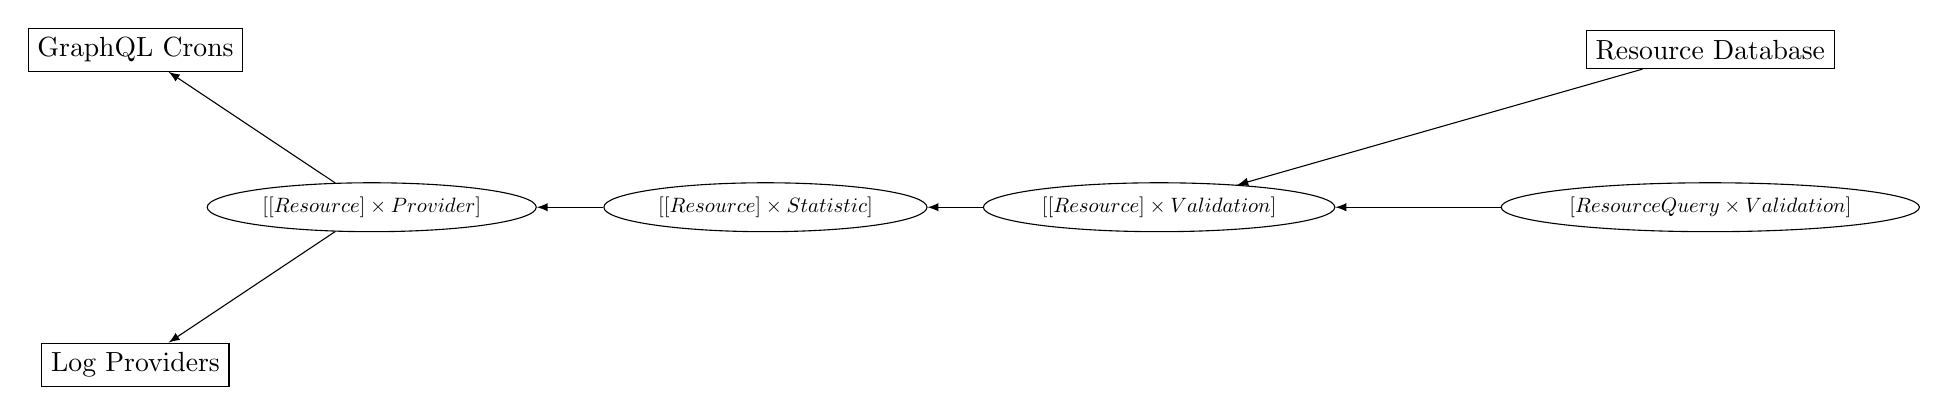
\begin{tikzpicture}
  \node[draw,ellipse,scale=0.75] (Query) at (0,0) {$[Resource Query \times Validation]$};
  \node[draw] (ResourceDatabase) at (0,2) {Resource Database};
  \node[draw,ellipse,scale=0.75] (Validations) at (-7,0) {$[[Resource] \times Validation]$};
  \node[draw,ellipse,scale=0.75] (Statistics) at (-12,0) {$[[Resource] \times Statistic]$};
  \node[draw,ellipse,scale=0.75] (Providers) at (-17,0) {$[[Resource] \times Provider]$};
  \node[draw] (LogFilters) at (-20,-2) {Log Providers};
  \node[draw] (GraphQLCrons) at (-20,2) {GraphQL Crons};

  \draw[-latex] (Query) -- (Validations);
  \draw[-latex] (ResourceDatabase) -- (Validations);
  \draw[-latex] (Validations) -- (Statistics);
  \draw[-latex] (Statistics) -- (Providers);
  \draw[-latex] (Providers) -- (LogFilters);
  \draw[-latex] (Providers) -- (GraphQLCrons);
\end{tikzpicture}
\end{document}
